\documentclass[11pt,a4paper,oneside]{book}

\usepackage{cmap}

\ifdefined\RUSSIAN
\usepackage[english,russian]{babel}
\usepackage[T2A]{fontenc}
\else
\usepackage[russian,english]{babel}
\usepackage[T2A]{fontenc}
\usepackage[default]{sourcesanspro}
\fi

\usepackage[utf8]{inputenc}
\usepackage{listings}
\usepackage{ulem}
\usepackage{url}
\usepackage{graphicx}
\usepackage{listingsutf8}
\usepackage[cm]{fullpage}
\usepackage{color}
\usepackage{fancyvrb}
\usepackage{xspace}
\usepackage{framed}
\usepackage{ccicons}
\usepackage{amsmath}
\usepackage[table]{xcolor}% http://ctan.org/pkg/xcolor
\usepackage[]{hyperref} % should be last

\definecolor{lstbgcolor}{rgb}{0.94,0.94,0.94}
\newcommand{\TT}[1]{\texttt{#1}}
\newcommand{\IT}[1]{\textit{#1}}
\newcommand{\IFRU}[2]{\iflanguage{russian}{#1}{#2}}
\newcommand{\forexample}{\IFRU{Например}{For example}:}
	

\newcommand{\TITLE}{\IFRU{Tracer: руководство пользователя}
{Tracer: users' manual}}
\newcommand{\AUTHOR}{\IFRU{Денис Юричев}{Dennis Yurichev}}
\newcommand{\EMAIL}{dennis@yurichev.com}

\hypersetup{
    pdftex,
    colorlinks=true,
    allcolors=blue,
    pdfauthor={\AUTHOR},
    pdftitle={\TITLE}
    }

\selectlanguage{english}

\lstset{
    backgroundcolor=\color{lstbgcolor},
    basicstyle=\ttfamily\footnotesize,
    breaklines=true,
    frame=single,
    inputencoding=cp1251,
    columns=fullflexible,keepspaces,
}

\begin{document}

\VerbatimFootnotes

\frontmatter

\begin{titlepage}
\begin{center}
\vspace*{\fill}
\LARGE \TITLE

\vspace*{\fill}

\large \AUTHOR

\large \TT{<\EMAIL>}
\vspace*{\fill}
\vfill

\ccbyncnd

\textcopyright 2013, \AUTHOR. 

\IFRU{Это произведение доступно по лицензии Creative Commons «Attribution-NonCommercial-NoDerivs» 
(«Атрибуция — Некоммерческое использование — Без производных произведений») 3.0 Непортированная. 
Чтобы увидеть копию этой лицензии, посетите}
{This work is licensed under the Creative Commons Attribution-NonCommercial-NoDerivs 3.0 Unported License. 
To view a copy of this license, visit} \url{http://creativecommons.org/licenses/by-nc-nd/3.0/}.

\IFRU{Дата компиляции этой PDF}{This PDF compilation date}: {\large \today}.

\IFRU{Англоязычная версия текста (а также сам tracer) также доступна по ссылке}{Russian language version of this text (as well as tracer itself) is also accessible at} \url{http://yurichev.com/tracer}
\end{center}
\end{titlepage}

\tableofcontents
\cleardoublepage

\chapter{\IFRU{Введение}{Preface}}

\IFRU{Tracer это win32-отладчик командной строки для выполнения простых отладочных задач.}{Tracer is command-line win32-debugger for performing simple debugging tasks.}

\IFRU{Главные возможности}{Major features}:

\begin{itemize}
\item \IFRU{Установка прерывания выполнении функции, вывод аргументов функции и результата}{Set breakpoint on function execution, track function arguments and result}.
\item \IFRU{Трассировка каждой инструкции функции и сохранение значений регистров}{Tracing each instruction of function and dumping register states}.
\item \IFRU{Установка прерывания в любом месте, вывод состояния регистров процессора и возможность изменить их}{Set breakpoint on arbitrary point, track CPU registers state and alter them}.
\item \IFRU{Установка прерывания на обращение к любой ячейки памяти и перехват всех обращений к ней}{Set breakpoint on memory cell access and track all accesses to it}.
\end{itemize}

\IFRU{Второстепенные возможности}{Minor features}:

\begin{itemize}
\item \IFRU{Установка прерывания задавая адрес, имя символа или байтмаски}{Set breakpoint by address, symbol name or bytemask}.
\item \IFRU{Обнаружение юникодных строк в аргументах функций}{Unicode string detection in function arguments}.
\item \IFRU{Поддержка как Windows x86 так и Windows x64}{Both Windows x86 and Windows x64 support}.
\item \IFRU{Поддержка символов Oracle RDBMS .SYM}{Oracle RDBMS .SYM files support}.
\item \IFRU{Наличие исходных кодов}{Source code included}.
\end{itemize}



\mainmatter

\chapter{\IFRU{Общие опции}{General options}}

\TT{-l:<fname.exe>}: \IFRU{загрузка процесса}{load process}.

\TT{-c:<cmd\_line>}: \IFRU{задание командной строки для загружаемого процесса}{define command line for loading process}.

\forexample{}

\begin{lstlisting}
tracer.exe -l:bzip2.exe -c:--help
\end{lstlisting}

\IFRU{Если командная строка содержит пробелы}{If command line contain spaces:}:

\begin{lstlisting}
tracer.exe -l:rar.exe "-c:a archive.rar *"
\end{lstlisting}

\TT{-a:<fname.exe|PID>}: \IFRU{присоединение к запущенному процессу по его имени или PID}{attach to running process by file name or PID number}.

\IFRU{Процесс с таким именем должен быть загружен. Если процессов с таким имененем загружено несколько, tracer присоеденяется ко всем сразу одновременно.}{Process with that filename should be already loaded. If there're several processes with the same name, tracer will attach to all of them simultaneously.}

\TT{--loading}: \IFRU{вывод имен файлов и базовых адресов для всех загружаемых модулей (обычно, это DLL-файлы).}{dump all module filenames and base addresses while loading (it's DLL files often).}

\TT{--child}: \IFRU{присоеденяться в том числе и к процессам порождаемых главным процессом}{attach to all child processes too}.

\IFRU{Например, вы можете запустить \TT{tracer.exe --child -l:cmd.exe}, откроется консольное окно cmd.exe и tracer будет присоеденятся к каждому процессу запущенному внутри командного интерпретатора.}{For example, you could run \TT{tracer.exe --child -l:cmd.exe}, this will open console cmd.exe window and every process running inside command interpreter will be handled by tracer.}

\TT{--allsymbols[:<regexp>]}: \IFRU{вывод всех символов в процессе загрузки по регулярному выражению}{dump all symbols during load or by regular expression}:

\TT{--allsymbols:somedll.dll!.*} \IFRU{опция может быть использована для вывода всех символов в некоторой DLL}{can be used for dumping all symbols in some DLL}.

\TT{--allsymbols:.*printf} \IFRU{выведет что-то вроде}{will print something like this}:

\begin{lstlisting}
New symbol. Module=[ntdll.dll], address=[0x77C004BC], name=[_snprintf]
New symbol. Module=[ntdll.dll], address=[0x77B8E61F], name=[_snwprintf]
...
New symbol. Module=[msvcrt.dll], address=[0x75725F37], name=[vswprintf]
New symbol. Module=[msvcrt.dll], address=[0x75726649], name=[vwprintf]
New symbol. Module=[msvcrt.dll], address=[0x756C3D68], name=[wprintf]
\end{lstlisting}

\TT{-s}: \IFRU{вывод стека вызовов перед каждым прерыванием}{dump call stack before each breakpoint}.

\forexample{}

\TT{tracer.exe -l:hello.exe -s bpf=kernel32.dll!WriteFile,args:5}

\IFRU{Мы увидим}{We will see}:

\begin{lstlisting}
23B4 (0) KERNEL32.dll!WriteFile (7, "hello to tracer!\r\n", 0x0000000E, 0x0017E3A4, 0) (called from 0x7317754E (MSVCR90.dll!_lseeki64+0x56b))
Call stack of thread 0x23B4
return address=731778D8 (MSVCR90.dll!_write+0x9f)
return address=7313FB4A (MSVCR90.dll!_fdopen+0x1c0)
return address=7313F70C (MSVCR90.dll!_flsbuf+0x6e1)
return address=73141E50 (MSVCR90.dll!printf+0x84)
return address=0040100E (hello.exe!BASE+0x100e)
return address=0040116F (hello.exe!BASE+0x116f)
return address=76FCE4A5 (KERNEL32.dll!BaseThreadInitThunk+0xe)
return address=77C9CFED (ntdll.dll!RtlCreateUserProcess+0x8c)
return address=77C9D1FF (ntdll.dll!RtlCreateProcessParameters+0x4e)
23B4 (0) KERNEL32.dll!WriteFile -> 1
\end{lstlisting}

\IFRU{Вывод стека вызова очень удобен, например, мы имеем программу показывающую окно с сообщением и перехватывая вызов \TT{USER32.DLL!MessageBoxA} мы можем увидеть путь к этому вызову.}{Stack dump can be very handy, for example, we have a program showing Message Box once and by intercepting \TT{USER32.DLL!MessageBoxA} call we can see a path to this call.}

\IFRU{Возможность вывода стека доступна для всех типов прерываний BPF/BPX/BPM.}{Stack dump feature available for all BPF/BPX/BPM features.}

\IFRU{Замечание: эта возможность пока не очень хорошо работает в x64.}{Note: this feature doesn't working in x64 version very well (yet).}

%*
\IFRU{Если указана опция \IT{--dump-fpu}, состояние регистров FPU будут показываться там где это возможно.}{If \TT{--dump-fpu} option is set, FPU registers state will be dumped wherever it's possible.}
%*
\IFRU{Если указана опция \IT{--dump-xmm}, состояние всех регистров XMM также будут выводиться, если только регистр не пуст.}{If \TT{--dump-xmm} option is set, each XMM registers state will be dumped (if needed) too, unless it is empty.}

%*
\TT{-t}: \IFRU{записывать дату и время перед каждой строкой в лог:}{write timestamp at each log line:}

\forexample{}

\begin{lstlisting}
tracer.exe -l:bzip2.exe bpf=cygwin1.dll!fprintf,args:2 -t
\end{lstlisting}

\begin{lstlisting}
[2013-07-03 07:15:10:056] TID=13056|(0) cygwin1.dll!fprintf (0x611887b0, "%s: For help, type: `%s --help'.\n") (called from bzip2.exe!OEP+0x15f1 (0x4025f1))
[2013-07-03 07:15:10:058] TID=13056|(0) cygwin1.dll!fprintf () -> 0x27
\end{lstlisting}

\IFRU{Эта возможность полезна тогда, когда нужно записывать в журнал время каких-то событий, например, когда именно некая программа обращается к сети.}{This feature is useful when one need to log time of some events into journal, like, when exactly some program accessed network.}

%*
\TT{--help}: \IFRU{помощь.}{print help.}
%*
\TT{-q}: \IFRU{запрет любого вывода в консоль и лог.}{be quiet, no output to console and log file.}

\TT{@}: \IFRU{опция позволяет сохранить все опции в текстовом файле и использовать их многократно:}{option can be used along with any other options:}

\begin{lstlisting}
tracer.exe @filename
\end{lstlisting}

\IFRU{Каждая строка файла представляет опцию. Это очень удобно для длинных и/или часто используемых опций, как байтмаски (смотрите ниже).}{Each line in the profile represents an option. This can be handy for lengthy and/or often used options, like bytemasks (see below).}

\IFRU{Опция \TT{@} также может использоваться с любыми другими опциями:}{\TT{@} option can be used along with any other options:}

\begin{lstlisting}
tracer.exe -l:filename.exe @additional_options @even_more_options
\end{lstlisting}



\chapter{\IFRU{Как в tracer задается адрес}{How address is defined in tracer}}

\IFRU{Имеется три возможности задать адрес прерывания.}{There're 3 ways to define breakpoint address.}

\begin{itemize}

\item \IFRU{Используя шестнадцатиричный адрес}{By hexadecimal address}: 
\TT{0x00400000} --- \IFRU{так задается абсолютный адрес внутри win32-процесса}
{that's how address inside of win32-process is to be set}.
\IFRU{Обратите внимание, что изменение базы
загрузки PE-модуля не учитывается, так что, если, например, в IDA, или ином дизассемблере, вы видите один адрес,
то этот код все же може быть загружен по другим адресам в памяти процесса 
(вы можете использовать опцию \TT{--loading}, чтобы увидеть,
по каким базовым адресам загружаются модули).}
{Please note: loading base changing of PE-module is not working out here, so,
if you see some address in IDA or any other disassembler, that piece of code may be loaded to another address in
memory process (you can use \TT{--loading} options to see, on which base address modules are being loaded).}

\IFRU{А для того, чтобы указать некий адрес в определенном PE-модуле, адрес должен быть задан так}{So, to set
some arbitrary address in specific PE-module, it should be set as}: 
\TT{module.dll!0x400000} --- \IFRU{и это адрес автоматически подкорректируется, 
если модуль будет загружен по другому базовому адресу}{and this address will be corrected automatically if module
will be loaded on another base address}.

\item \IFRU{Используя символ}{By symbol}.

\forexample{} \TT{kernel32.dll!writefile}

\IFRU{Здесь можно использовать регулярные выражения.
Например: \TT{.*!printf</i>}: tracer будет искать символ \TT{printf} в каждом загружаемом модуле. Если этот символ имеется в разных модулях, tracer будет использовать только из того модуля, который был загружен раньше всех.}
{Regular expressions can be used here.
For example: \TT{.*!printf}: tracer will look for \TT{printf} symbol in each loading module. If the same name occurs in different modules, tracer will use only the first occurence.}

\IFRU{Для регулярных выражений используется синтаксис POSIX Extended Regular Expression (ERE)}{POSIX Extended Regular Expression (ERE) syntax is used here for regular expressions}.

\IFRU{Из-за того что здесь задается регулярное выражение, некоторые символы, такие как \TT{?}, \TT{.} нужно 
\IT{escape-ть}.
Например, чтобы задать адрес \TT{?method@class@@QAEHXZ}, нужно указывать \TT{\textbackslash{}?method@class@@QAEHXZ}.}
{Since this is regular expression, some symbols, like \TT{?}, \TT{.} should be \IT{escaped}. 
For example, in order to set \TT{?method@class@@QAEHXZ} address, it should be set as \TT{\textbackslash{}?method@class@@QAEHXZ}.}

\IFRU{Смещение также можно использовать. Например: \TT{file.exe!BASE+0x1234} (BASE это предопределенный символ, он равен базовому адресу PE-модуля) либо \TT{file.exe!label+0xa}.}{Offset is allowed here. For example: \TT{file.exe!BASE+0x1234} (base is predefined symbol equals to PE file base) or \TT{file.exe!label+0xa}.}

\begin{comment}
\item \IFRU{Используя байтмаску}{By bytemask}.

\IFRU{Иногда нужна возможность установить прерывание внутри модуля по шаблону, например такому, какие используются в сигнатурах IDA.}{Sometimes, we would like to define breakpoint inside of an executable by byte pattern, just like IDA signature.}

\forexample{}

\begin{lstlisting}
tracer.exe -l:cycle.exe bpf=558BEC8B45085068........FF15........83C4085DC3,args:1
\end{lstlisting}

\IFRU{tracer будет искать этот шаблон во всех исполняемых секциях каждого загружаемого модуля и будет выводить:}{tracer will look for this pattern in each executable section of each loading module and will print:}

\begin{lstlisting}
===============================================================================
cycle.exe: searching for bytemask_0 in .text section...
bytemask_0 is resolved to address 0x00401000 (cycle.exe)
===============================================================================
\end{lstlisting}

\IFRU{Две точки вместо двух шестнадцатиричных цифр означают \IT{любой байт}. Это очень удобно для пропуска FIXUP-ов, итд.}{Two dots instead of two hexadecimal digits mean \IT{any byte}. This can be useful for skipping FIXUPs, etc.}

\IFRU{Возможно также указать \TT{[skip:n]} для пропуска нескольких байт внутри байтмаски, например: \TT{55[skip:10]1100} эквивалентно \TT{bpf=55....................1100}.}{It is also possible to mention \TT{[skip:n]} to skip several bytes during bytemask search, for example: \TT{55[skip:10]1100} --- this is equivalent to \TT{bpf=55....................1100}.}

\IFRU{Замечание: обычно, если байтмаской задается функция, то достаточно определить только начало функции.}{Note: if some function is defined by bytemask, only bytes from the beginning of function are enough.}

\IFRU{Замечание: байтмаска может встречаться много раз в одном и том же модуле. tracer предупредит об этом, но будет использовать только первую найденную. Это значит что байтмаска для функции должна задаваться аккуратно.}{Note: bytemask can appear more than once in one module. tracer will warn us on, and use only the first occurence by default. This means that function byte pattern is to be constructed accurately.}
\end{comment}

\end{itemize}


\chapter{\IFRU{BPF: установка прерывания на исполнение функции}{BPF: set breakpoint on function execution}}

\IFRU{Опция BPF, в каком-то смысле, похожа на работу утилиты}{BPF option, in a way, it is a kind of} strace\footnote{\url{http://en.wikipedia.org/wiki/Strace}}.

\IFRU{Главные отличия от strace:}{Significant differences with strace are:}

\begin{itemize}
\item tracer \IFRU{работает только в win32/win64.}{is win32/win64 only.}
\item \IFRU{Прерыванием может быть любоая функция а не только системные вызовы.}{Breakpoints not just system calls, but any function.}
\item \IFRU{Только 4 прерывания из-за ограничений архитектуры x86.}{Only 4 breakpoints, because of x86 architecture limitation.}
\end{itemize}

\IFRU{BPF с адресом но без дополнительных опций будет только показывать момент вызова функции и то что она возвращает.}{BPF option with address without additional options will only track the moment when function was called and what it returns.}

\forexample{}

\begin{lstlisting}
tracer.exe -l:bzip2.exe bpf=kernel32.dll!WriteFile
\end{lstlisting}

\begin{lstlisting}
1188 (0) KERNEL32.dll!WriteFile () (called from 0x610AC912 (cygwin1.dll!sigemptyset+0x1022))
1188 (0) KERNEL32.dll!WriteFile -> 1
\end{lstlisting}

\IFRU{Замечание: tracer не знает о том что функция может иметь тип \IT{void} (т.е., не возвращает ничего). Таким образом, tracer выводит просто то что находится в регистре \TT{EAX}/\TT{RAX} на момент выхода из функции.}{Note: tracer doesn't know some function is void type, e.g., it doesn't return any value. So it just takes the value at \TT{EAX}/\TT{RAX} register.}

\IFRU{Опции}{Options}:

\TT{ARGS:<number>}: \IFRU{определить количество агрументов для перехватываемой функции}{define arguments number for the function we would like to intercept}.

\forexample{}

\begin{lstlisting}
tracer.exe -l:bzip2.exe -c:--help bpf=kernel32.dll!WriteFile,args:5
\end{lstlisting}

\begin{lstlisting}
09D0 (0) KERNEL32.dll!WriteFile (0x0000001B, "   If no file names are given, bzip2 compresses or decompresses", 0x0000003F, "?", 0)
09D0 (0) KERNEL32.dll!WriteFile -> 1
09D0 (0) KERNEL32.dll!WriteFile (0x0000001B, "   from standard input to standard output.  You can combinesses", 0x0000003B, ";", 0)
09D0 (0) KERNEL32.dll!WriteFile -> 1
09D0 (0) KERNEL32.dll!WriteFile (0x0000001B, "   short flags, so `-v -4' means the same as -v4 or -4v, &amp;c.ses", 0x0000003C, "<", 0)
09D0 (0) KERNEL32.dll!WriteFile -> 1
\end{lstlisting}

\IFRU{То что мы видим это попытку вывести 5 агрументов функции при каждом вызове функции WriteFile().}{What we see here is an attempt to read 5 arguments at each WriteFile function call.}
\IFRU{Если аргумент является указателем в пределах памяти процесса и то на что он указывает может быть интерпретировано как ASCII-строка, она будет выведена.}{If some of these arguments are pointers to some area within process memory, and the data at the pointer can be interpreted as ASCII string, it will be printed instead.}
\IFRU{Это очень удобно для перехвата строковых функций таких как strcmp(), strlen(), strtok(), atoi(), итд.}{This is useful when intercepting string functions like strcmp(), strlen(), strtok(), atoi(), and so on.}

\IFRU{Ошибится в количестве аргументов не страшно (кроме случая использования опции \TT{skip\_stdcall}, смотрите ниже). Если указанное количество аргументов больше чем на самом деле, возможно, значения из локальных переменных вызывающей функции будут выведены. Или какой-нибудь случайный мусор. Если заданное количество аргументов меньше чем на самом деле, только часть аргументов будет выведена.}{It is not a problem to make mistake on arguments number (except using \TT{skip\_stdcall} option, see below). If defined arguments number greater than real, captured local variables of caller function probably will be printed. Or any other useless junk. If defined arguments number is less than real, then only part of arguments will be visible.}

\TT{RT:<number>}: \IFRU{подставить другое возвращаемое значение в момент выхода из функции, на лету.}{replace the returning value of any function by something else, on fly.}

\begin{lstlisting}
tracer.exe -l:filename.exe bpf=function,args:1,rt:0x12345678
\end{lstlisting}

tracer \IFRU{запишет это значение в регистр \TT{EAX}/\TT{RAX} в момент выхода из функции.}{will put this value to \TT{EAX}/\TT{RAX} right at the moment when function exited.}

\TT{SKIP}: \IFRU{пропустить выполнение функции. Эта опция может использоваться вместе с опцией \TT{RT}.}{bypass a function. This can be used with \TT{RT} option too.}

\begin{lstlisting}
tracer.exe -l:filename.exe bpf=function,args:1,rt:0x12345678,skip
\end{lstlisting}

\IFRU{Это означает что в момент начала выполнения функции, управление сразу будет передано на выход и возвращаемое значение будет установлено в 0x12345678.}{This means that the function just gets bypassed and its return value is fixed at 0x12345678.}

\IFRU{Замечание: без префикса "0x", это значение будет интерпретироваться как десятичное число.}{Note: without "0x" prefix, this value would be interpreted as decimal number.}

\TT{SKIP\_STDCALL}: \IFRU{то же что и \TT{SKIP}, только для stdcall-функций.}{the same as <b>SKIP</b> option but rather used for stdcall functions.}

\IFRU{Разница между типами функций cdecl и stdcall в том что функция типа сdecl на выходе не выравнивает указатель стека (вызывающая функция должна сделать это). Функция типа stdcall выравнивает указатель стека. cdecl это наиболее используемый тип функций. Хотя, stdcall используется в MS Windows. Так что, если вы хотите пропустить выполнение какой-либо функции в KERNEL32.DLL или USER32.DLL, вы должны использовать \TT{skip\_stdcall}. Следовательно, в этом случае, tracer должен знать точное количество аргументов, а без этого процесс может упасть.}{The difference between cdecl and stdcall calling conventions is just that cdecl function doesn't align stack pointer at exit (caller should do this). stdcall function aligns stack pointer at exit. cdecl is the most used calling convention. However, stdcall is used in MS Windows. So, if you would like to skip a function in KERNEL32.DLL or USER32.DLL, you should use \TT{skip\_stdcall}. Consequently, in this case, tracer must know the exact arguments number, without it the process may crash.}\footnote{\IFRU{Смотрите также}{See also}: X86 calling conventions\url{http://en.wikipedia.org/wiki/X86_calling_conventions}}

\IFRU{Если вы хотите подавить все вызовы функции WriteFile:}{If you'd like to suppress all WriteFile calls, do this:}

\begin{lstlisting}
tracer.exe -l:hello.exe bpf=kernel32.dll!WriteFile,args:5,skip_stdcall,rt:1
\end{lstlisting}

\IFRU{Не забывайте возвращать 1, для того чтобы вызываемая функция не заподозрила ничего!}{Don't forget to make it return 1, so the caller will not suspect anything!}
\IFRU{Количество аргументов функции WriteFile --- 5. Поменяйте это значение на что-то другое и процесс упадет.}{WriteFile arguments number is just 5. Change it to something different, and process crashes.}

\IFRU{Замечание: тип функции stdcall отсутствует в Windows x64, так что эта опция отсутствует в 64-битной версии tracer.}{Note: stdcall calling convention is absent in Windows x64, so this option is absent in win64-version of tracer.}

\TT{UNICODE}: \IFRU{трактовать строки в аргументах как юникодные (два байта на каждый символ). Это может быть полезно для перехвата win32-функций с суффиксом W, например, MessageBoxW.}{treat strings in arguments as unicode (widechar). This could be helpful if you intercept unicode win32 functions with W suffix, for example, MessageBoxW.}

\IFRU{К сожалению, tracer умеет автоматически выявлять только строки использующие первую половину таблицы ASCII, так что строки на других языках кроме тех что используют латиницу не будут выявлены автоматически.}{Unfortunately, tracer can only automatically detect first half of ASCII table, so multilingual unicode strings will not be detected.}

\TT{DUMP\_ARGS:<size>}: \IFRU{дампить память по аргументам функции (если она чиается) с ограничением size.}{dump memory on argument (if readable) limited by max size.}

\IFRU{Если аргумент функции содержит указатель на читаемый блок памяти, он будет выведен.}{If argument contain pointer to valid memory block, it will be printed.}

\IFRU{На момент выхода из функции, если блок в памяти изменился, то разница будет выведена также.}{At the function exit, if memory block contents was changed, difference will be printed too.}

\forexample{}

\begin{lstlisting}
tracer64.exe -l:test_getlocaltime.exe bpf=.*!getlocaltime,args:1,dump_args:0x30
\end{lstlisting}

\begin{lstlisting}
TID=6660|(0) KERNEL32.dll!GetLocalTime (0x12ff00) (called from 0x14000100f (getlocaltime.exe!BASE+0x100f))
Dump of buffer at argument 1 (starting at 1)
000000000012FF00: 28 FF 12 00 00 00 00 00-00 00 00 00 00 00 00 00 "(..............."
000000000012FF10: 01 00 00 00 00 00 00 00-73 11 00 40 01 00 00 00 "........s..@...."
000000000012FF20: 00 00 00 00 00 00 00 00-00 00 00 00 00 00 00 00 "................"
TID=6660|(0) KERNEL32.dll!GetLocalTime -> 0x150
Dump difference of buffer at argument 1 (starting at 1)
0000000000000000: D9 07 0C    06    05   -05    10    24    50 01 "... . . . . $ P."
\end{lstlisting}

\IFRU{Таким образом мы можем увидеть как win32-функция GetLocalTime() заполняет структуру SYSTEMTIME.}{Now we can see how GetLocalTime win32 function fill SYSTEMTIME structure.}

\section{\IFRU{Опция TRACE}{TRACE option}}

\TT{TRACE}: \IFRU{трассировать функцию по одной инструкции и сохранять значения всех интересующих нас регистров. После исполнения, эта информация сохранится в файлы process.exe.idc, process.exe.txt, process.exe\_clear.idc. .idc-файлы являются скриптами для IDA, а к .txt файлу можно применять grep, awk, sed для поиска интересующих нас значений.}{trace each instruction in function and collect all interesting values from registers and memory. After execution, all that information is saved to process.exe.idc, process.exe.txt, process.exe\_clear.idc files. .idc-files are IDA scripts, .txt file is grepable by grep, awk and sed.}

\IFRU{Возьмем для примера функцию add\_member из статьи}{For example, let's take add\_member function from} \IT{Using Uninitialized Memory for Fun and Profit}\footnote{\url{http://research.swtch.com/2008/03/using-uninitialized-memory-for-fun-and.html}}\IFRU{}{article}:

\begin{lstlisting}
int dense[256];
int dense_next=0;
int sparse[256];

void add_member(int i)
{
	dense[dense_next]=i;
	sparse[i]=dense_next;
	dense_next++;

};

int main ()
{
	add_member(123);
	add_member(5);
	add_member(71);
	add_member(99);
}
\end{lstlisting}

\IFRU{Скомпилируем и запустим трассировку на функции add\_member (вначале узнайте адрес функции при помощи IDA):}{Let's compile it and run tracing on add\_member function (determine function address in IDA before):}

\begin{lstlisting}
tracer -l:trace_test4.exe bpf=0x00401000,trace:cc
\end{lstlisting}

\IFRU{Получим файл trace\_test4.exe.txt:}{We'll get trace\_test4.exe.txt file:}

\begin{lstlisting}
0x401000, e=       4
0x401001, e=       4
0x401003, e=       4, [0x403818]=0..3
0x401008, e=       4, [EBP+8]=5, 0x47('G'), 0x63('c'), 0x7b('{')
0x40100b, e=       4, ECX=5, 0x47('G'), 0x63('c'), 0x7b('{')
0x401012, e=       4, [EBP+8]=5, 0x47('G'), 0x63('c'), 0x7b('{')
0x401015, e=       4, [0x403818]=0..3
0x40101a, e=       4, EAX=0..3
0x401021, e=       4, [0x403818]=0..3
0x401027, e=       4, ECX=0..3
0x40102a, e=       4, ECX=1..4
0x401030, e=       4
0x401031, e=       4, EAX=0..3
\end{lstlisting}

\IFRU{Поле \IT{e} - это сколько раз была исполнена эта инструкция.}{\IT{e} field is how many times was executed this instruction.}

\IFRU{Загрузим trace\_test4.exe.idc в IDA и увидим:}{Let's execute trace\_test4.exe.idc script in IDA and we'll see:}

\begin{figure}[ht!]
\centering
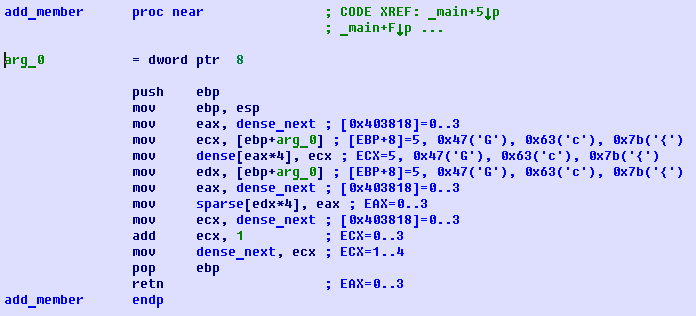
\includegraphics[scale=0.66]{trace_test4.png}
\caption{trace\_test4.png}
\end{figure}

\IFRU{Понимать работу функции во время исполнения, таким образом, становится намного проще.}{Now it is much simpler to understand how this function work during execution.}

\IFRU{Исполненные инструкции подсвечиваются голубым цветом. Неисполненные остаются белыми.}{Executed instructions are highlighed by blue color. Not-executed instructions are leaved white.}

\IFRU{Чтобы стереть все комментарии и подсветку, нужно исполнить скрипт trace\_test4.exe\_clear.idc}{If you need to clear all comments and highlight, execute trace\_test4.exe\_clear.idc script.}

\IFRU{Информация в IDA-скрипте может приводится в сокращенной форме из-за того что IDA имеет ограничение на длину комментария, например: \TT{EAX=[ 64 unique items. min=0xbca6eb7, max=0xffffffed ]}. В текстовом же файле сохраняется всё, поэтому иногда этот файл может оказаться в итоге очень большим.}{All collected information in IDA-script may be reduced to shorten form like \IT{EAX=[ 64 unique items. min=0xbca6eb7, max=0xffffffed ]} (because IDA has comment size limitation). On contrary, everything is saved to text file without shortening, that is why resulting text file may be sometimes pretty big.}

\IFRU{Недостаток опции TRACE в том что она работает медленно, хотя и функции в системных DLL пропускаются (системной считается та DLL которая находится внутри \%SystemRoot\%) Вторая проблема в том что пока что не очень корректно трассируются вещи вроде исключений, setjmp/longjmp и подобных непредвиденных изменений пути исполнения кода.}{One problem of TRACE feature that it is slow, however, functions from system DLLs are skipped (system DLL is that DLL residing in \%SystemRoot\%) Another problem is that things like exceptions, setjmp/longjmp and other unexpected codeflow alterations are not correctly handled so far.}



\section{\IFRU{Примеры}{Examples}}

\subsection{\IFRU{Простое использование}{Simple usage}}

\begin{lstlisting}
tracer.exe -l:bzip2.exe bpf=.*!fprintf,args:3
\end{lstlisting}

\begin{lstlisting}
TID=5128|(0) cygwin1.dll!fprintf (0x61103150, "%s: I won't write compressed data to a terminal.\n", "bzip2") (called from 0x401e03 (bzip2.exe!BASE+0x1e03))
TID=5128|(0) cygwin1.dll!fprintf -> 0x34
TID=5128|(0) cygwin1.dll!fprintf (0x61103150, "%s: For help, type: `%s --help'.\n", "bzip2") (called from 0x401c66 (bzip2.exe!BASE+0x1c66))
TID=5128|(0) cygwin1.dll!fprintf -> 0x27
\end{lstlisting}

\subsection{\IFRU{Перехват некоторых Windows-функций для работы с реестром}{Intercept some Windows registry access functions}}

\begin{lstlisting}
tracer.exe -l:someprocess.exe bpf=advapi32.dll!RegOpenKeyExA,args:5 bpf=advapi32.dll!RegQueryValueExA,args:6 bpf=advapi32.dll!RegSetValueExA,args:6
\end{lstlisting}

.. \IFRU{или измените суффиксы функция на W и добавьте опцию UNICODE}{or change function suffixes to W and add UNICODE option}:

\begin{lstlisting}
tracer64.exe -l:far.exe bpf=advapi32.dll!RegOpenKeyExW,args:5,unicode bpf=advapi32.dll!RegQueryValueExW,args:6,unicode bpf=advapi32.dll!RegSetValueExW,args:6,unicode
\end{lstlisting}

\subsection{\IFRU{Подавить шумный сигнал}{Suppress noisy beeping}}

\begin{lstlisting}
tracer.exe -l:beeper.exe bpf=kernel32.dll!Beep,args:2,skip_stdcall,rt:1
\end{lstlisting}

\subsection{\IFRU{Подавить диалоговое окно с сообщением}{Suppress Message Box}}

... \IFRU{и сделать так что вызываемая функция будет считать что пользователь каждый раз нажимает OK (константа IDOK равняется 1)}{by making it appear to a caller that the user presses OK every time (IDOK constant is 1)}:

\begin{lstlisting}
tracer.exe -l:filename.exe bpf=user32.dll!MessageBoxA,args:4,skip_stdcall,rt:1
\end{lstlisting}

... \IFRU{или CANCEL (константа IDCANCEL равняется 2)}{or CANCEL (IDCANCEL constant is 2)}:

\begin{lstlisting}
tracer.exe -l:filename.exe bpf=user32.dll!MessageBoxA,args:4,skip_stdcall,rt:2
\end{lstlisting}

\subsection{\IFRU{Перехват вызовов rand()}{Intercepting rand() call}}

\IFRU{Бывает весело перехватывать вызовы функции rand() в различных играх. Например, пасьянс Solitaire в Windows использует его для того чтобы сгенерировать случайный расклад. Мы можем установить возвращаемое значение rand() в ноль, и тогда Solitaire будет раздавать один и тот же расклад, всегда:}{Another fun is intercepting rand() function in various games. For example, Windows Solitaire card game use it to generate random deal. We can fix rand() return at zero, and Solitaire will do the same deal each time, forever:}

\IFRU{В}{In} Windows XP x86/x64:

\begin{lstlisting}
tracer.exe/tracer64.exe -l:c:\windows\system32\sol.exe bpf=.*!rand,rt:0
\end{lstlisting}

\IFRU{В}{In} Windows 7 x64:

\begin{lstlisting}
tracer64.exe -l:[full path to]\Solitaire.exe bpf=.*!rand,rt:0
\end{lstlisting}

\subsection{FreeCell}

\IFRU{Когда вы запускаете FreeCell в Windows (XP SP3) и нажимаете F2 (Новая игра), вы видите сообщение "Do you want to resign this game?" Мы можем подавить звуковой сигнал и сделать так что FreeCall будет думать что пользователь всегда нажимает YES:}{When you run Windows (XP SP3) FreeCell and press F2 (New game), you will get a message box "Do you want to resign this game?" We can suppress all that beeping and also make illusion to FreeCell user always press YES:}

\IFRU{Константа IDYES - 6. FreeCell использует функцию MessageBoxW - суффикс W означает уникодную версию функции MessageBox.}{IDYES constant is 6. FreeCell use MessageBoxW - W mean unicode version of MessageBox.}

\IFRU{В}{In} Windows XP SP3 x86:

\begin{lstlisting}
tracer.exe -l:c:\windows\system32\freecell.exe bpf=user32.dll!messagebeep,args:1,skip_stdcall bpf=user32.dll!messageboxw,args:4,unicode,skip_stdcall,rt:6
\end{lstlisting}

\begin{lstlisting}
TID=444|(0) USER32.dll!MessageBeep (0x20) (called from 0x1001f52 (freecell.exe!BASE+0x1f52))
We skip execution of this function
TID=444|(1) USER32.dll!MessageBoxW (0x80122, L"Do you want to resign this game?", L"FreeCell", 0x24) (called from 0x1001f5f (freecell.exe!BASE+0x1f5f))
We skip execution of this function
TID=444|We modify return value (EAX) of this function to 6
\end{lstlisting}

\IFRU{В}{In} Windows XP SP2 x64 Russian:

\begin{lstlisting}
tracer64.exe -l:c:\windows\system32\freecell.exe bpf=user32.dll!messagebeep,args:1,skip bpf=user32.dll!messageboxw,args:4,unicode,skip,rt:6
\end{lstlisting}

\begin{lstlisting}
TID=2028|(0) USER32.dll!MessageBeep (0x20) (called from 0x1000023f9 (freecell.exe!BASE+0x23f9))
We skip execution of this function
TID=2028|(1) USER32.dll!MessageBoxW (0x1f00f0, 0xbf80, 0xbf20, 0x24) (called from 0x100002416 (freecell.exe!BASE+0x2416))
We skip execution of this function
TID=2028|We modify return value (RAX) of this function to 6
\end{lstlisting}

\subsection{\IFRU{Проверка ивентов и запись в лог в Oracle RDBMS}{Oracle RDBMS Events checking and log writes}}

\IFRU{В}{In} Oracle 10.2.0.1 win64:

\begin{lstlisting}
tracer64.exe -a:oracle.exe bpf=oracle.exe!ksdpec,args:1 bpf=oracle.exe!ss_wrtf,args:3
\end{lstlisting}

( \IFRU{Смотрите также}{See also}: \url{http://blog.yurichev.com/node/14} )

\begin{lstlisting}
TID=3032|(0) oracle.exe!ksdpec (0x2743) (called from 0x9580a9 (oracle.exe!opiodr+0x105))
TID=3032|(0) oracle.exe!ksdpec -> 0xff
TID=3032|(1) oracle.exe!ss_wrtf (0x4a0, "*** 2009-12-04 06:19:01.005\n", 0x1b) (called from 0x45318d (oracle.exe!sdpri+0x22d))
TID=3032|(1) oracle.exe!ss_wrtf -> 1
TID=3032|(1) oracle.exe!ss_wrtf (0x4a0, "OPI CALL: type=107 argc= 3 cursor=  0 name=SES OPS (80)\n", 0x37) (called from 0x45318d (oracle.exe!sdpri+0x22d))
TID=3032|(1) oracle.exe!ss_wrtf -> 1
TID=3032|(0) oracle.exe!ksdpec (0x2743) (called from 0x9580a9 (oracle.exe!opiodr+0x105))
TID=3032|(0) oracle.exe!ksdpec -> 0xff
TID=3032|(1) oracle.exe!ss_wrtf (0x4a0, "OPI CALL: type=59 argc= 4 cursor=  0 name=VERSION2\n", 0x32) (called from 0x45318d (oracle.exe!sdpri+0x22d))
TID=3032|(1) oracle.exe!ss_wrtf -> 1
TID=3032|(0) oracle.exe!ksdpec (0x273e) (called from 0x4a00cc (oracle.exe!kslwte_tm+0x7a8))
TID=3032|(0) oracle.exe!ksdpec -> 0
TID=3032|(0) oracle.exe!ksdpec (0x273e) (called from 0x4a00cc (oracle.exe!kslwte_tm+0x7a8))
TID=3032|(0) oracle.exe!ksdpec -> 0
TID=3032|(0) oracle.exe!ksdpec (0x2743) (called from 0x9580a9 (oracle.exe!opiodr+0x105))
TID=3032|(0) oracle.exe!ksdpec -> 0xff
TID=3032|(1) oracle.exe!ss_wrtf (0x4a0, "OPI CALL: type=104 argc=12 cursor=  0 name=Transaction Commit/Rollback\n", 0x46) (called from 0x45318d (oracle.exe!sdpri+0x22d))
TID=3032|(1) oracle.exe!ss_wrtf -> 1
\end{lstlisting}

\subsection{\IFRU{Слежение за выделением памяти в}{Trace memory allocations in} Oracle 11.1.0.6.0 win32/win64}

\begin{lstlisting}
tracer.exe/tracer64.exe -a:oracle.exe bpf=.*!kghalf,args:6 bpf=.*!kghfrf,args:4
\end{lstlisting}

\begin{lstlisting}
TID=1600|(0) oracle.exe!kghalf (0x6d35af0, 0xb507ef8, 0x1000, 0, 0, "kzsrcrdi") (called from 0x1c7aa83 (oracle.exe!kzctxhugi+0x71))
TID=1600|(0) oracle.exe!kghalf -> 0xfa3ea58

TID=1600|(0) oracle.exe!kghalf (0x6d35af0, 0xb507ef8, 0x58, 1, 0x6d35530, "UPI heap") (called from 0x1e7f8b7 (oracle.exe!__PGOSF266_kwqmahal+0x5b))
TID=1600|(0) oracle.exe!kghalf -> 0xfa4d0d8

TID=1188|(0) oracle.exe!kghalf (0xda39540, 0xda39240, 0x88, 0, "ksirmdt array", 0xda39240) (called from 0x6afb5b (oracle.exe!ksz_nfy_ipga+0xf1))
TID=1188|(0) oracle.exe!kghalf -> 0x105d0b10

TID=1188|(0) oracle.exe!kghalf (0xda39540, 0xda39240, 0x48, 1, 0x1204e400, "local") (called from 0x3684a64 (oracle.exe!kjztcxini+0x58))
TID=1188|(0) oracle.exe!kghalf -> 0x105d0ab0
\end{lstlisting}

\subsection{\IFRU{Слежение за разбором SQL-выражений в}{SQL statements parsing in} Oracle RDBMS}

\IFRU{В}{In} Oracle 11.1.0.6.0 win32/win64:

\begin{lstlisting}
tracer.exe/tracer64.exe -a:oracle.exe bpf=oracle.exe!_?rpisplu,args:8 bpf=oracle.exe!_?kprbprs,args:7 bpf=oracle.exe!_?opiprs,args:6 bpf=oraclient11.dll!OCIStmtPrepare,args:6</i></p>
\end{lstlisting}

\IFRU{Замечание: регулярное выражение \IT{\_?function} покрывает оба имени: \TT{function} и \TT{\_function}.}{Note: regular expression \TT{\_?function} cover both \TT{function} and \TT{\_function}.}

\begin{lstlisting}
TID=1140|(2) oracle.exe!opiprs (0x13f029d0, "select 1 from obj$ where name='DBA_QUEUE_SCHEDULES'", 0x34, 0x10ae7f50, 0x840082, 0xd9f7a10) (called from 0x6ba3bf (oracle.exe!__PGOSF423_kksParseChildCursor+0x2dd))
TID=1140|(2) oracle.exe!opiprs -> 0
TID=1140|(2) oracle.exe!opiprs (0x13f029d0, "select 1 from sys.aq$_subscriber_table where rownum < 2 and subscriber_id <> 0 and table_objno <> 0", 0x64, 0x10ad5de8, 0, 0x13f007e0) (called from 0x6ba3bf (oracle.exe!__PGOSF423_kksParseChildCursor+0x2dd))
TID=1140|(2) oracle.exe!opiprs -> 0
TID=1140|(0) oracle.exe!rpisplu (3, 0, 0, 0, 0, 0x14430ac0, 0, 0) (called from 0x250b33c (oracle.exe!kqdGetCursor+0x106))
TID=1140|(0) oracle.exe!rpisplu -> 0
TID=1288|(2) oracle.exe!opiprs (0x17df8130, "select * from v$version", 0x18, 0x10adee60, 0, 0) (called from 0x6ba3bf (oracle.exe!__PGOSF423_kksParseChildCursor+0x2dd))
TID=1288|(1) oracle.exe!kprbprs (0xa82bc50, 0, "select timestamp, flags from fixed_obj$ where obj#=:1", 0x35, 0xffffe3e0, 0x2040800, 1) (called from 0x2ba1b1f (oracle.exe!kqldtstr+0x151))
TID=1288|(1) oracle.exe!kprbprs -> 0
TID=1288|(0) oracle.exe!rpisplu (0x1f, 0, 0, 0, 0, 0x2bb5e04, "select  BANNER from GV$VERSION where inst_id = USERENV('Instance')", 0xffffc085) (called from 0x2bbcabf (oracle.exe!kqldFixedTableLoadCols+0x157))
TID=1288|(1) oracle.exe!kprbprs (0x1090c108, 0, "select timestamp, flags from fixed_obj$ where obj#=:1", 0x35, 0xffffe3e0, 0x2040800, 1) (called from 0x2ba1b1f (oracle.exe!kqldtstr+0x151))
TID=1288|(1) oracle.exe!kprbprs -> 0
TID=1288|(1) oracle.exe!kprbprs (0x10908060, 0, "select timestamp, flags from fixed_obj$ where obj#=:1", 0x35, 0xffffe3e0, 0x2040800, 1) (called from 0x2ba1b1f (oracle.exe!kqldtstr+0x151))
TID=1288|(1) oracle.exe!kprbprs -> 0
TID=1288|(2) oracle.exe!opiprs -> 0
TID=1288|(0) oracle.exe!rpisplu -> 0
TID=1288|(0) oracle.exe!rpisplu (0x16, 0, 0, 0, 0, 0x10b3ce50, 0, 0) (called from 0x250b33c (oracle.exe!kqdGetCursor+0x106))
TID=1288|(0) oracle.exe!rpisplu -> 0
\end{lstlisting}

\subsection{\IFRU{Игнорирование неподписанных драйверов}{Ignore unsigned drivers}}

\begin{lstlisting}
tracer.exe -l:target.exe bpf=Wintrust.dll!WinVerifyTrust,rt:0
\end{lstlisting}

\subsection{\IFRU{Вывод памяти по аргументам функций}{Dump function arguments}}

\begin{lstlisting}
tracer.exe -l:rar.exe "-c:a archive.rar *.exe" bpf=kernel32.dll!writefile,args:5,dump_args:0x10
\end{lstlisting}

\IFRU{RAR записывает свою сигнатуру в начало файла archive.rar:}{RAR writting its signature to the beginning of archive.rar file:}

\begin{lstlisting}
TID=7000|(0) KERNEL32.dll!WriteFile (0x118, 0x152410, 7, 0x150fc0, 0) (called from 0x403721 (rar.exe!__GetExceptDLLinfo+0x26c8))
Dump of buffer at argument 2 (starting at 1)
00152410: 52 61 72 21 1A 07 00 00-50 30 15 00 5D 83 40 00 "Rar!....P0..].@."
Dump of buffer at argument 4 (starting at 1)
00150FC0: 00 00 00 00 21 7B 40 00-10 24 15 00 18 24 15 00 "....!{@..$...$.."
TID=7000|(0) KERNEL32.dll!WriteFile -> 1
\end{lstlisting}

\subsection{\IFRU{Вывод памяти по аргументам функций и слежение за её изменением}{Dump function arguments and track difference occured in buffers}}

\begin{lstlisting}
tracer.exe -l:rar.exe "-c:x archive.rar" bpf=kernel32.dll!readfile,args:4,dump_args:0x10
\end{lstlisting}

\IFRU{Архиватор RAR открывает файл archive.rar и первым делом читает сигнатуру:}{RAR archiver open archive.rar and read signature for the first:}

\begin{lstlisting}
TID=6148|(0) KERNEL32.dll!ReadFile (0x120, 0x17b3f8, 7, 0x174c50) (called from 0x403966 (rar.exe!__GetExceptDLLinfo+0x290d))
Dump of buffer at argument 2 (starting at 1)
0017B3F8: 00 00 00 00 00 00 00 00-00 00 00 00 48 00 00 00 "............H..."
Dump of buffer at argument 4 (starting at 1)
00174C50: 07 00 00 00 78 4C 17 00-7A 38 40 00 8C 6D 17 00 "....xL..z8@..m.."
TID=6148|(0) KERNEL32.dll!ReadFile -> 1
Dump difference of buffer at argument 2 (starting at 1)
00000000: 52 61 72 21 1A 07      -                        "Rar!..          "
\end{lstlisting}



\section{\IFRU{Примеры опции TRACE}{TRACE feature examples}}

\subsection{\IFRU{Трассировка строковых функций}{Tracing string functions}}

\IFRU{Возьмем пример применения strtok():}{Let's take strtok() example:}

\begin{lstlisting}
// example from http://www.cplusplus.com/reference/clibrary/cstring/strtok/

/* strtok example */
#include <stdio.h>
#include <string.h>

int main ()
{
  char str[] ="- This, a sample string.";
  char * pch;
  printf ("Splitting string \"%s\" into tokens:\n",str);
  pch = strtok (str," ,.-");
  while (pch != NULL)
  {
    printf ("%s\n",pch);
    pch = strtok (NULL, " ,.-");
  }
  return 0;
}
\end{lstlisting}

\IFRU{И трассируем функцию main():}{Let's trace main() function:}

\begin{lstlisting}
tracer.exe -l:trace_test1.exe bpf=0x00401000,trace:cc
\end{lstlisting}

\IFRU{После исполнения скрипта в IDA (показана только тело цикла \IT{while}):}{After executing resulting .idc script in IDA (only \IT{while} loop body showed here):}

\begin{figure}[ht!]
\centering
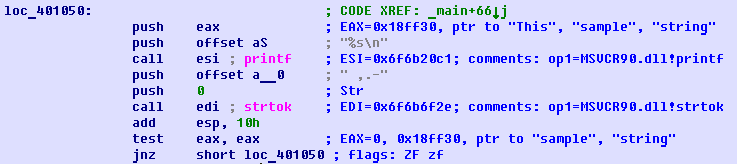
\includegraphics[scale=0.66]{trace_test1.png}
\caption{trace\_test1.png}
\end{figure}

\IFRU{Замечание: "a" это слишком короткая строка для автоматического детектора строк в tracer, поэтому её здесь нет, вместо нее адрес этой строки.}{Note: "a" is too short string for automatic string detector in tracer, that is why it is absent and its address here instead.}

\subsection{\IFRU{Трассируем quicksort()}{Let's trace quicksort()}}

\IFRU{Возьмем известный пример:}{Use well-known example:}

\begin{lstlisting}
//http://cplus.about.com/od/learningc/ss/pointers2_8.htm

/* ex3 Sorting ints with qsort */
//

#include <stdio.h>
#include <stdlib.h>

int comp(const int * a,const int * b) 
{
  if (*a==*b)
    return 0;
  else
    if (*a < *b)
        return -1;
     else
      return 1;
}

int main(int argc, char* argv[])
{
   int numbers[10]={1892,45,200,-98,4087,5,-12345,1087,88,-100000};
   int i;

  /* Sort the array */
  qsort(numbers,10,sizeof(int),comp);
  for (i=0;i<9;i++)
    printf("Number = %d\n",numbers[ i ]);
  return 0;
}
\end{lstlisting}

\IFRU{Трассируем функцию comp():}{Let's trace comp() function:}

\begin{lstlisting}
tracer.exe -l:trace_test2.exe bpf=0x00401030,trace:cc
\end{lstlisting}

\IFRU{Получим после исполнения скрипта в IDA:}{We will get after .idc script execution in IDA:}

\begin{figure}[ht!]
\centering
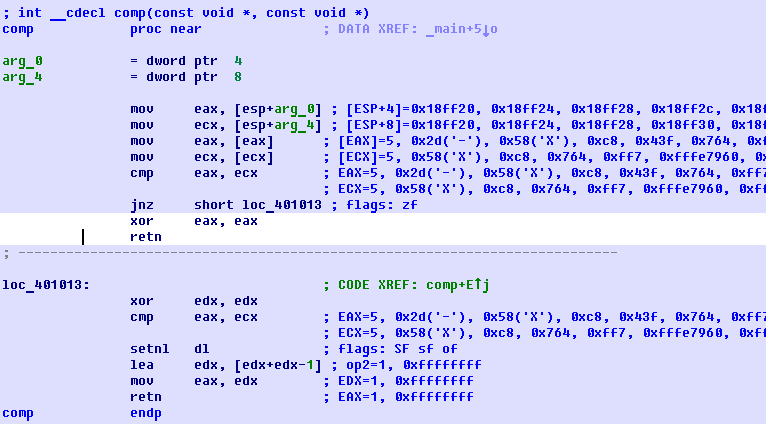
\includegraphics[scale=0.66]{trace_test2.png}
\caption{trace\_test2.png}
\end{figure}

\IFRU{В примере все значения уникальны, одинаковых нет. Таким образом, нет ситуации когда comp() возвращает ноль. Поэтому здесь мы видим что часть comp() возвращающая ноль (xor eax,eax / retn) не была исполнена ни разу.}{In this example all values are unique, there are no equal ones. Therefore, there are no situation when comp() function returning zero. That is why we see that the comp() part returning zero (xor eax,eax / retn) was not executed.}





\chapter{\IFRU{BPX: установка прерывания на произвольное место}{BPX: set breakpoint arbitrary point}}

\IFRU{Содержимое регистров процессора будет выведено.}{Content of all CPU registers will be printed.}

\IFRU{Если хотя бы один регистр FPU что-то содержит, он также будет выведен.}{If at least one FPU register contain something, it will be printed too.}

\IFRU{Если содержимое FPU-регистра NaN (нечисло), содержимое регистра FPU будет трактовано как регистра MMX и также будет выведено.}{If the floating point number is also NaN (Not-a-Number), FPU register contents will be treated as MMX register and will be dumped too.}

\IFRU{\TT{DUMP(ADDRESS|REGISTER|SYMBOL[+OFFSET],SIZE)}: вывод содержимого памяти. Определить адрес в памяти можно в виде шестнадцатиричного значения или в виде \TT{REGISTER+OFFSET}. \TT{SIZE} --- это размер дампа.}{\TT{DUMP(ADDRESS|REGISTER[+OFFSET],SIZE)}: dump contents of memory. Define memory address by hexadecimal address or in form \TT{REGISTER+OFFSET}. \TT{SIZE} is memory dump size.}

\IFRU{Если перед адресом или регистром поставить символ \TT{*}, то tracer вначале прочитает DWORD (или QWORD в x64-версии), примет его за адрес и выдаст дамп по нему. Например: \TT{dump(*ebx,0x100)} --- взять адрес из ячейки памяти на которую указывает регистр ebx и выдать дамп размером 0x100 байт.}{If an asteriks symbol \TT{*} is set before address or register value, then tracer will read DWORD (or QWORD in x64 version), treat it as address and dump a buffer here. For example: \TT{dump(*ebx,0x100)} --- take address on a memory cell EBX register pointing on and dump buffer with size of 0x100 bytes.}

\IFRU{\TT{COPY(ADDRESS|REGISTER|SYMBOL[+OFFSET],C-string)}: скопировать Си-строку по указанному адресу. Си-строка может быть как ASCII-строкой, так и содержать последовательности \TT{\textbackslash{}xXX}, где \TT{XX} --- шестнадцатиричное число. Например: \TT{COPY(EAX,a\textbackslash{}x34\textbackslash{}x56)} --- скопирует три байта 'a', 0x34, и 0x56 по адресу который содержится в EAX.}{\TT{COPY(ADDRESS|REGISTER|SYMBOL[+OFFSET],C-string)}: copy C-string to that address. C-string can be just ASCII-string, but also may contain such sequences like \TT{\textbackslash{}xXX}, where \TT{XX} --- hexadecimal number. For example: \TT{COPY(EAX,a\textbackslash{}x34\textbackslash{}x56)} --- copy 3 bytes 'a', 0x34, and 0x56 to address from EAX register.}

\IFRU{\TT{SET (REGISTER,VALUE)}: записать значение в регистр. EIP/RIP, регистры FPU ST0..ST7 и флаги (PF, SF, AF, ZF, OF, CF, DF) можно модифицировать. Значение трактуется как десятичное число или как число с плавающей запятой, если только не указан префикс 0x.}{\TT{SET (REGISTER,VALUE)}: set register to value. EIP/RIP, FPU registers ST0..ST7 and flags (PF, SF, AF, ZF, OF, CF, DF) are allowed. Value will be treated as decimal or floating point, unless prefix 0x is present.}

\IFRU{Замечание: tracer не модифицирует tag word register в FPU, также он не модифицирует регистр TOP, таким образом, если какой-то регистр FPU маркирован как "пустой" и tracer запишет туда какое-то значение, он останется маркированным как "пустой".}{Note: tracer never modify FPU tag word register as well as not modify TOP register, so, if some FPU register was marked as "empty" and tracer set some value there, it will remain marked "empty".}

\IFRU{Изменение значения регистра EIP/RIP иными словами это передача исполнения в другое место. Это удобно для того чтобы пропускать некоторые куски кода.}{Changing EIP/RIP is on other words is code flow altering. This is useful to bypass some code pieces.}

\section{\IFRU{Примеры}{Examples}}

\subsection{\IFRU{Task Manager: создать иллюзию что у нас 32 или 64 процессора}{Task Manager: make illusion we have 32 or 64 CPUs}}

\IFRU{В}{In} Windows XP SP2 x64 Russian:

\begin{lstlisting}
tracer64.exe -l:c:\windows\system32\taskmgr.exe bpx=0x000000010000A8E4,set(rax,64)
\end{lstlisting}

\IFRU{В}{In} Windows XP SP3 x86 English:

\begin{lstlisting}
tracer.exe -l:c:\windows\system32\taskmgr.exe bpx=0x01006647,set(eax,32)
\end{lstlisting}

\subsection{\IFRU{Перехват развернутой (inline) функции strcmp()}{Inlined strcmp() intercepting}}

\IFRU{Представим что у нас есть такой код который мы компилируем в MS VC 2008:}{Let's imagine we have a code we compile in MS VC 2008:}

\begin{lstlisting}
printf ("%d\n", strcmp("one", "two"));
\end{lstlisting}

\IFRU{После компиляции мы получим:}{After compiling we got:}

\begin{lstlisting}
<pre>
.text:00401000 BA 50 A1 40 00                    mov     edx, offset aTwo ; "two"
.text:00401005 B9 54 A1 40 00                    mov     ecx, offset aOne ; "one"
.text:0040100A 8D 9B 00 00 00 00                 lea     ebx, [ebx+0]
.text:00401010
.text:00401010                   loc_401010:                             ; CODE XREF: _main+2A
.text:00401010 8A 01                             mov     al, [ecx]
.text:00401012 3A 02                             cmp     al, [edx]
.text:00401014 75 29                             jnz     short loc_40103F
.text:00401016 84 C0                             test    al, al
.text:00401018 74 12                             jz      short loc_40102C
.text:0040101A 8A 41 01                          mov     al, [ecx+1]
.text:0040101D 3A 42 01                          cmp     al, [edx+1]
.text:00401020 75 1D                             jnz     short loc_40103F
.text:00401022 83 C1 02                          add     ecx, 2
.text:00401025 83 C2 02                          add     edx, 2
.text:00401028 84 C0                             test    al, al
.text:0040102A 75 E4                             jnz     short loc_401010
.text:0040102C
.text:0040102C                   loc_40102C:                             ; CODE XREF: _main+18
.text:0040102C 33 C0                             xor     eax, eax
.text:0040102E 50                                push    eax
.text:0040102F 68 58 A1 40 00                    push    offset byte_40A158 ; char *
.text:00401034 E8 1C 00 00 00                    call    _printf
.text:00401039 83 C4 08                          add     esp, 8
.text:0040103C 33 C0                             xor     eax, eax
.text:0040103E C3                                retn
\end{lstlisting}

\IFRU{Давайте перехватим эту развернутую функцию strcmp и выведем то на что указывают регистры ECX и EDX:}{Let's intercept inlined strcmp function and dump what is at ECX and EDX:}

\begin{lstlisting}
tracer.exe -l:strcmp.exe bpx=8A013A02752984C074128A41013A4201751D83C10283C20284C075E433C0,dump(ecx,0x10),dump(edx,0x10)
\end{lstlisting}

\IFRU{Получим:}{We got:}

\begin{lstlisting}
bytemask_0 is resolved to address 0x401010 (strcmp.exe)
TID=6436|(0) 0x401010 (strcmp.exe!BASE+0x1010)
EAX=0x007722E0 EBX=0x7EFDE000 ECX=0x0040A154 EDX=0x0040A150
ESI=0x00000000 EDI=0x00000000 EBP=0x0018FF88 ESP=0x0018FF44
EIP=0x00401010
FLAGS=PF ZF IF
Dumping memory at ECX
0040A154: 6F 6E 65 00 25 64 0A 00-28 00 6E 00 75 00 6C 00 "one.%d..(.n.u.l."
Dumping memory at EDX
0040A150: 74 77 6F 00 6F 6E 65 00-25 64 0A 00 28 00 6E 00 "two.one.%d..(.n."
\end{lstlisting}

\IFRU{Замечание: только первое вхождение при поиске байтмаски будет использоваться.}{Note: only first bytemask occurence will be intercepted.}

\subsection{\IFRU{Изменение флагов перед тем как условный переход будет совершен}{Change flags before conditional dump is taken}}

\begin{lstlisting}
tracer64.exe -l:flags.exe bpx=0x140001014,set(zf,1)
\end{lstlisting}

\IFRU{Замечание: момент когда tracer меняет состояние регистров это момент \IT{перед} тем как текущая инструкция будет исполнена. Изменение флагов \IT{перед} инструкциями TEST или CMP бессмысленно.}{Note: the moment when tracer can change registers state is the moment \IT{before} current instruction is executed. Changing flags \IT{before} TEST or CMP instructions is useless.}

\subsection{\IFRU{Шутка в Microsoft Excel}{Microsoft Excel practical joke}}

\IFRU{Сделать 666 результатом всех операций деления. Введите "=(123/456)" для проверки.}{Make result of all divisions 666. Enter "=(123/456)" to check.}

\IFRU{Работает для Excel.exe версии}{Works for Excel.exe version} 14.0.4756.1000 (Microsoft Office 2010)

\begin{lstlisting}
tracer.exe -l:excel.exe bpx=excel.exe!base+0x11E91B,set(st0,666)
\end{lstlisting}

\begin{lstlisting}
tracer64.exe -l:excel.exe bpx=excel.exe!base+0x1B7FCC,set(st0,666)
\end{lstlisting}

\IFRU{(Указанный адрес это место после инструкции FDIV, которая собственно и производит деление)}{(The address there is the point after FDIV instruction actually do division here)}

\begin{figure}[ht!]
\centering
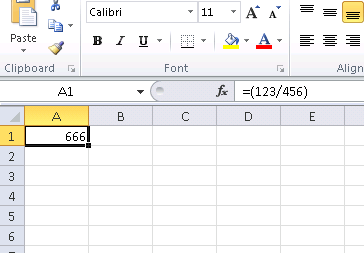
\includegraphics[scale=0.66]{excel_prank.png}
\caption{excel\_prank.png}
\end{figure}



\chapter{\IFRU{BPM: установка прерывания на обращение к ячейке памяти}{BPM: set breakpoint on memory access}}

\IFRU{Архитектура x86 позволяет устанавливать прерывания на обращение к ячейкам памяти.}{x86 architecture allows to set breakpoints on a memory value access.}

\IFRU{Таким образом, если кто-то или что-то модифицирует в памяти какое-то значение, tracer тут же будет об этом знать.}{That is, if someone or something modifies some value, gt will be instantly notified.}

\IFRU{Следует также заметить, что это практично только для глобальных переменных а не локальных (размещаемых в стеке).}{It is also should be noted that these breakpoints only practical for global variables, not local ones (stored in stack).}

\TT{BPMB=<address>,<option>}: \IFRU{установить прерывание на обращение к байту.}{set breakpoint on byte value access.}
\TT{BPMW=<address>,<option>}: \IFRU{установить прерывание на обращение к 16-битному слову (word).}{set breakpoint on 16-bit word value access.}

\TT{BPMD=<address>,<option>}: \IFRU{установить прерывание на обращение к 32-битному слову (dword).}{set breakpoint on 32-bit dword value access.}

\TT{BPMQ=<address>,<option>}: \IFRU{установить прерывание на обращение к 64-битному слову (qword) (доступно только в tracer64).}{set breakpoint on 62-bit qword value access (available only in tracer64).}

\TT{W}: \IFRU{установить прерывание только на запись в ячейку памяти.}{set breakpoint only on memory value write.}

\TT{RW}: \IFRU{установить прерывание на запись и чтение из ячейки памяти.}{set breakpoint on both memory value read/write.}

\IFRU{Замечание: по какой-то неизвестной причине, архитектура Intel предоставляет только две эти возможности.}{Note: because of some unknown reason, Intel achitecture offers only these two opportunities.}

\section{\IFRU{Примеры}{Examples}}

\subsection{\IFRU{Слежение за обращением к переменным в Oracle RDBMS}{Tracing value access in Oracle RDBMS}}

\IFRU{Давайте попробуем следить за всеми чтениями и записями в глобальную переменную ktsmgd и видеть стек вызовов:}{Let's trace read-write access to ktsmgd global variable and see call stack:}

\begin{lstlisting}
tracer.exe -a:oracle.exe -s bpmd=oracle.exe!_?ktsmgd_,rw
\end{lstlisting}

\IFRU{Запустите в консоли SQL*Plus (залогиньтесь перед этим как SYS):}{Run in SQL*Plus console (login as SYS before):}

\begin{lstlisting}
ALTER SYSTEM SET "_disable_txn_alert"=1;
\end{lstlisting}

\IFRU{Получим:}{We got:}

\begin{lstlisting}
TID=2852|(0) oracle.exe!_ktsmgdcb+0x18: some code reading or writting DWORD variable at oracle.exe!_ktsmgd_ (now it contain 0x1)
Call stack of thread TID=2852
return address=0x4682f0 (oracle.exe!_kspptval+0x704)
return address=0x4674b0 (oracle.exe!_kspset0+0x928)
return address=0x8f23c6 (oracle.exe!_kkyasy+0x3cda)
return address=0x92ba1d (oracle.exe!_kksExecuteCommand+0x475)
return address=0x1f75e02 (oracle.exe!_opiexe+0x4bda)
return address=0x1e98390 (oracle.exe!_kpoal8+0x900)
return address=0x9df597 (oracle.exe!_opiodr+0x4cb)
return address=0x6102eb00 (oracommon11.dll!_ttcpip+0xab0)
return address=0x9de77e (oracle.exe!_opitsk+0x4fe)
return address=0x1fdf128 (oracle.exe!_opiino+0x430)
return address=0x9df597 (oracle.exe!_opiodr+0x4cb)
return address=0x450b1c (oracle.exe!_opidrv+0x32c)
return address=0x451352 (oracle.exe!_sou2o+0x32)
return address=0x401197 (oracle.exe!_opimai_real+0x87)
return address=0x401061 (oracle.exe!_opimai+0x61)
return address=0x401c55 (oracle.exe!_OracleThreadStart@4+0x301)
return address=0x77e66063 (KERNEL32.dll!GetModuleFileNameA+0xeb)
\end{lstlisting}

\IFRU{Читайте больше тут: \url{http://blog.yurichev.com/node/3} о параметре \TT{\_disable\_txn\_alert} и значении переменной \TT{ktsmgd}.}{Visit \url{http://blog.yurichev.com/node/3} for more information about \TT{\_disable\_txn\_alert} parameter and \TT{ktsmgd} value.}



\chapter{\IFRU{Взаимодействие во время работы}{Interacting while running}}

1) \IFRU{Нажмите ESC или Ctrl-C для отсоединения от запущенного процесса.}{Press ESC or Ctrl-C to detach from the running process.}

2) \IFRU{Нажмите пробел чтобы увидеть стеки вызовов для каждого треда и процесса.}{Press SPACE to see current call stacks for each thread of each process.}

\IFRU{Например: присоеденитесь к какой-нибудь запущенной программе с открытым окном с сообщением (Message Box), нажмите пробел и возможно вы увидите, что привело к появлению этого окна.}{For example: attach to some running application with opened Message Box, press SPACE and see what probably caused it.}

\IFRU{Замечание: вывод стека вызовов пока плохо работает в tracer64.}{Note: dump call stack feature is not very well working in tracer64.}

\chapter{\IFRU{Отсоединение от процесса}{Detaching}}

\IFRU{tracer использует функцию DebugActiveProcessStop() для отсоединения от запущенного процесса. Эта функция присутствует во всех современных ОС базирующихся на NT, возможно, кроме Windows NT и Windows 2000. Так что всё что tracer может сделать в этих ОС это убить процесс --- извините!}{tracer uses DebugActiveProcessStop() function to detach from the running process. It is present in all modern NT-based operation systems, probably, except Windows NT and Windows 2000. So all tracer can do is just to kill the running process --- sorry!}

\chapter{\IFRU{Некоторые технические заметки}{Some other technical notes}}

\IFRU{Архитектура x86 позволяет использовать до четырех прерываний одновременно. Таким образом, опции \TT{BPF/BPX/BPM} могут комбинироваться в любом порядке до четырех раз.}{x86 architecture allow to use up to 4 breakpoints simultaneously. So, \TT{BPF/BPX/BPM} features can be combined in any order up to 4 times.}

\IFRU{Возможность вывода стека вызовов предпологает что фреймы в стеке "разделены" указателем в регистре EBP:}{Stack dumping feature consider stack frames "divided" with EBP base pointer:}

\IFRU{Смотрите также}{See laos}: \href{http://en.wikibooks.org/wiki/X86_Disassembly/Functions_and_Stack_Frames}{Functions and Stack Frames}

\IFRU{Это означает что любая функция которая не использует эту схему, будет исключена их стека вызовов --- непреднамеренно.}{This means that any function which doesnt use this scheme will be excluded from stack dump --- unintentionally.}

\IFRU{Замечание: эта возможность отсутствует в tracer64.}{Note: this feature absent in tracer64.}

\IFRU{Вся информация выводится в stdout а также записывается в файл tracer.log. Файл создается снова при каждом запуске.}{All information dumped to stdout is also written to tracer.log file. This file is created at each start.}

\IFRU{При загрузке или присоеденению к процессу, tracer проверяет все модули: главный исполняемый файл и все файлы DLL загружаемые после. Он извлекает все символы из модуля включая эксплорты DLL. Он также ищует файл FileName.MAP и пытается его парсить. Файл MAP имеет такой же формат как то что делает IDA. tracer также ищет файл FileName.SYM и пытается загрузить символы из него, трактуя его как файл символов из Oracle RDBMS: переменная окружения ORACLE\_HOME должна быть установлена для этого. tracer также ищет файл FileName.PDB (компилируйте вашу программу в MSVC с ключом \TT{/Zi} и вы получите отладочный файл PDB для нее).}{While loading or attaching, tracer will inspect all modules: main executable and all DLL files loaded after. It will fetch all present symbols, incuding export entries of DLL files. It will also look for FileName.MAP file and try to parse information from it. MAP file has the same format as that produced by IDA disassembler. tracer will also look for FileName.SYM file and try to load symbols from it, treating those as Oracle RDBMS SYM file format: ORACLE\_HOME environment value should be set for this. tracer will also look for FileName.PDB file (compile your program in MSVC with \TT{/Zi} option and get debug PDB file for it).}

\IFRU{Если DLL содержит экспорты только по ординалам, т.е., без имен (например, DLL-файлы MFC), имя символа будет получено из ординала в таком формате: \TT{ordinal\_<number>}, например, \TT{ordinal\_12}.}{If DLL contain only exports by ordinals, e.g., without names (MFC DLLs, for example), the name of ordinal will be generated in compliance with \TT{ordinal\_<number>} format, for example, \TT{ordinal\_12}.}

\chapter{\IFRU{Заключение}{Conclusion}}

\IFRU{Эта версия еще не была протестирована как следует. Так что будьте готовы к неожиданным падениям. Я очень рекомендую проводить все эксперименты в виртуальной машине.}{This release is not tested properly yet. So please be prepared for any possible crash. I strongly advice to do all experimentation in virtual machine.}

\IFRU{Если вы нашли ошибку, пожалуйста напишите мне:}{If you find any bug, please drop me a line:} \href{mailto:dennis@conus.info}{dennis@conus.info}. \IFRU{Пришлите также файл tracer.log и/или скриншот того что вывел tracer.}{Please attach tracer.log file and screenshot of the last tracer output.}

\IFRU{Я буду также благодарен любому комментарию или предложению насчет tracer.}{I'll also be thankful for any comments and suggestions related to tracer tool.}

\IFRU{Если вы чувствуете что ваш вклад в код стоит того чтобы быть включенным в мою версию, пожалуйста присылайте ваш патч.}{If you feel your contribution to source code is worth enough, please send me your patch.}

\end{document}
